\documentclass[border=4pt]{standalone}
\usepackage{amsmath,amssymb,amsfonts}
\usepackage{xcolor,colortbl,array,booktabs,multirow}
\usepackage{tikz}
\usetikzlibrary{arrows, automata, backgrounds, calendar, chains, decorations,
    matrix, mindmap, patterns, petri, positioning, shadows, shapes.geometric,
    trees, shapes, decorations.pathreplacing, calc, tikzmark, arrows.meta}
\newcommand{\st}{\text{ s.t. }}
\newcommand{\x}{\mathbf{x}}
\renewcommand{\b}{\mathbf{b}}
\newcommand{\A}{\mathbf{A}}
\newcommand{\R}{\mathbb{R}}
\newcommand{\RR}{\mathbb{R}}
\newcommand{\Z}{\mathbb{Z}}
\newcommand{\ZZ}{\mathbb{Z}}
\begin{document}
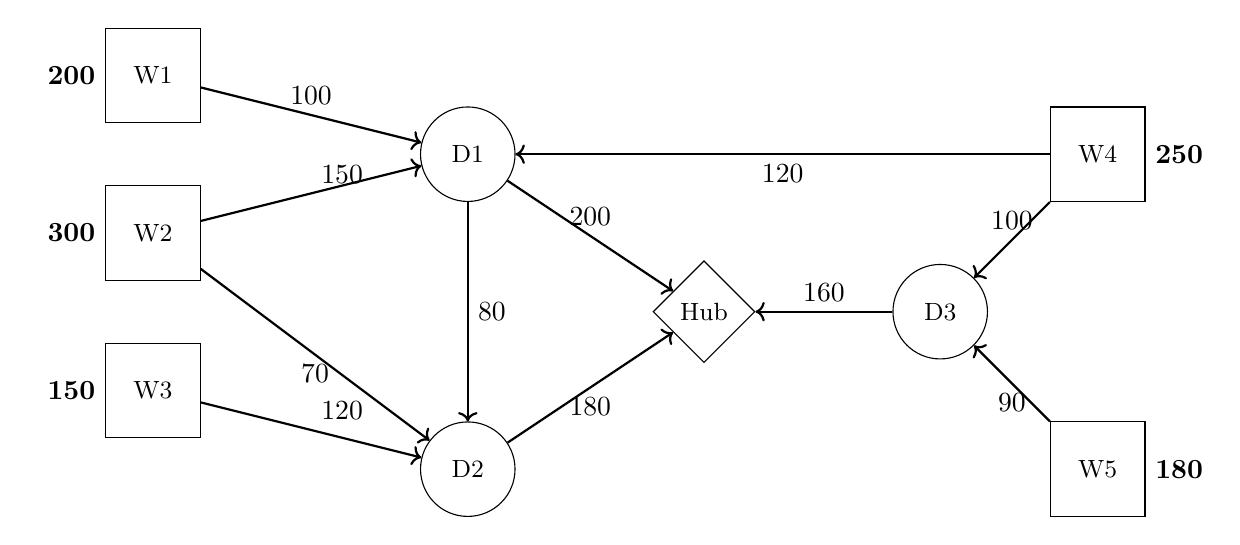
\begin{tikzpicture}[
    node distance=1.5cm and 2.5cm,
    warehouse/.style={draw, rectangle, minimum size=1.2cm, font=\small},
    distribution/.style={draw, circle, minimum size=1.2cm, font=\small},
    hub/.style={draw,  diamond, minimum size=1.2cm, font=\small}]

   % Nodes with inventory labels
    \node[warehouse, label=left:{\textbf{ 200}}] (W1) at (-4,3) {W1};
    \node[warehouse, label=left:{\textbf{300}}] (W2) at (-4,1) {W2};
    \node[warehouse, label=left:{\textbf{150}}] (W3) at (-4,-1) {W3};
    \node[distribution] (D1) at (0,2) {D1};
    \node[distribution] (D2) at (0,-2) {D2};
    \node[hub] (Hub) at (3,0) {Hub};
    \node[warehouse, label=right:{\textbf{250}}] (W4) at (8,2) {W4};
    \node[warehouse, label=right:{\textbf{180}}] (W5) at (8,-2) {W5};
    \node[distribution] (D3) at (6,0) {D3};

    % Arcs
    \draw[->, thick] (W1) -- node[above] {100} (D1);
    \draw[->, thick] (W2) -- node[above right] {150} (D1);
    \draw[->, thick] (W3) -- node[above right] {120} (D2);
    \draw[->, thick] (D1) -- node[above] {200} (Hub);
    \draw[->, thick] (D2) -- node[below] {180} (Hub);
    \draw[->, thick] (D1) -- node[right] {80} (D2);
    \draw[->, thick] (D3) -- node[above] {160} (Hub);
    \draw[->, thick] (W4) -- node[above] {100} (D3);
    \draw[->, thick] (W5) -- node[below] {90} (D3);
    \draw[->, thick] (W4) -- node[below] {120} (D1);
    \draw[->, thick] (W2) -- node[below] {70} (D2);\end{tikzpicture}
\end{document}
